% Chapter 8: Universal Gravitation: Apples, the Moon, and Tides
\chapter{Universal Gravity: Apples, the Moon, and Tides}

\step{A Counterintuitive Opening}

If you live by the sea or have watched it while traveling, you may have noticed something odd: the sea rises and falls twice daily, with a high tide a little more than twelve hours apart. Stranger still, when the Moon is overhead pulling up the water directly beneath it, water on Earth's far side, facing away from the Moon, also rises.

Stop and consider how counterintuitive this is. It is easy to picture the Moon pulling up water beneath it: gravity reaches through vacuum, pulls hardest on the nearest water, and raises a bulge there. But the far-side water is farthest from the Moon and pulled least strongly. Why should it bulge too? If gravity merely meant the Moon tugging seawater, the farthest water should be pulled flattest and have the day's lowest level. Reality says the opposite: near and far sides have high tide almost together, while the lowest levels occur between those directions.

This is no word game but an observation anyone can check: open a port city's tide timetable and you see two daily high tides about twelve hours and twenty-five minutes apart, not one. The Moon takes nearly a month to orbit Earth, which rotates once daily. Neither seems to yield two unless something is missing from our usual picture of gravity.

This chapter supplies that missing something. Explaining the far-side tide requires upgrading gravity from the Moon tugging objects to a pull that varies with distance. Tides arise from the difference between the pulls at Earth's near and far ends. Difference will become the second half's central word.

We begin with tides but will explain more: floating astronauts, communication satellites apparently fixed overhead, Voyager probes flung out of the solar system, and even your phone locating you within a few meters all rely on this same set of ideas.

\step{Make a Guess First}

Before reading on, honestly write your intuitive answers. No research needed; wrong guesses make it interesting.

Question one: water rises directly beneath the Moon and on Earth's opposite side. Is it because (a) lunar gravity goes around Earth to the other side; (b) Earth is pulled harder than the far-side water, relatively moving away from it; or (c) the Moon pushes Earth's atmosphere across and squeezes the water upward?

Question two: astronauts float in a space station because (a) it is so high that Earth's gravity is negligible; (b) vacuum has no air to support them, so they float; or (c) something else?

Question three: throw a stone horizontally from a tower. A harder throw lands farther away. If your strength could become unlimited, would the stone eventually (a) fly straight away into space forever; (b) circle Earth and hit the back of your head; or (c) always reach the ground, only farther away?

Question four: do an apple falling and the Moon orbiting Earth follow the same law or different laws?

Keep your answers. We will return to them individually at the end. If you chose (a) for question two, most people agree with you, and it is the classic wrong answer.

\step{Hands-on Experiment}

Our most important intuition is that something spreading uniformly in every direction becomes more dilute farther away. Gravity spreads this way. A flashlight and phone let you feel the idea at home.

\begin{experiment}[Why a Light Spot Gets Larger and Dimmer]
Turn off the room lights and shine your phone flashlight, or any flashlight, onto a white wall. Start with it against the wall and slowly move backward.

Two things happen together: the spot grows and dims. If it remains roughly circular, measure approximately. At twice the distance, its diameter roughly doubles and area quadruples, while brightness falls to about one-quarter. At three times the distance, area is about ninefold and brightness one-ninth.

If your phone can run a light-meter app, many free ones read its ambient-light sensor, fix the phone in place and move the flashlight away while recording readings. Brightness roughly falls as inverse distance squared: one-quarter at twice the distance, one-ninth at three times.

Why? The flashlight emits the same total light, spread over increasing area. Light from a small bulb travels straight outward in all directions, spreading like an inflating balloon's surface. Double a balloon's radius and its surface quadruples. Paint originally covering one patch must now cover four times that area, naturally becoming four times paler.

Clarify the analogy's resemblance and difference. Like light, gravity spreads uniformly outward from a source, so its dilution follows inverse distance squared. Unlike gravity, light is an energy flow that walls can block and absorb. Gravity is almost impossible to shield: you cannot insert a gravitational barrier between Moon and sea. Borrow only the geometry of spreading, not too much else.
\end{experiment}

A second experience needs a strong string about a meter long and an eraser. Tie the eraser to one end, swing it slowly overhead in a circle, then speed up. You clearly feel stronger tension on your hand at greater speed. Lengthen the string while keeping the same rotation rate and tension changes too. Your hand does what Earth does to the Moon: continually pulls the eraser inward through the string so it cannot fly straight away. Remember the feeling that circling needs a continuous inward pull. It is the key to orbits.

\step{The Old Model Runs into Trouble}

Before universal gravitation, how did people explain the world, and why did that explanation reach its limit?

The oldest, most natural view gave heaven and Earth separate rules. Terrestrial stones, apples, and water naturally fell downward and stopped at the ground, the nature of heavy things. Celestial moons, planets, and stars did not fall; they circled by nature. This account ruled for almost two thousand years because it fit everyday observation so closely: you never saw the Moon fall or an apple orbit anything.

Yet the two-rule model has a fatal weakness: it never answers why. Why should celestial objects circle and terrestrial objects fall? Keep asking and it can only say because that is their nature. Physics calls this rephrasing the question, not explaining it. Worse, it makes no quantitative predictions: it cannot say how many days a lunar orbit takes or how many tides occur daily.

A second problem comes from a thought experiment you can do now. Stand securely on a chair, or simply imagine it, holding a small pebble. Throw it horizontally and it arcs a few meters to the ground. Imagine twice the strength giving twice the distance. Continue to a kilometer, ten, a hundred: something subtle happens. Earth is round, and as the stone flies forward, the ground curves downward below it. Fast enough, each forward stretch sees the ground recede by exactly the amount the stone falls. It forever approaches the ground without reaching it, falling continually without landing. It has begun orbiting Earth.

This is Newton's famous mountaintop cannon. Fire horizontally from a high mountain: faster shots land farther away, and at a certain speed the shot never lands at all. The essential point is that it has not escaped falling but keeps falling. Every second of its orbit it drops toward the ground, which keeps avoiding it.

\begin{center}
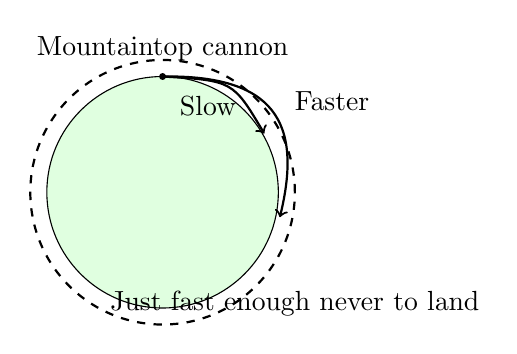
\begin{tikzpicture}[scale=1.05]
  \fill[green!12] (0,0) circle (1.4);
  \draw (0,0) circle (1.4);
  \fill (0,1.4) circle (1.2pt);
  \node[above=2pt] at (0,1.4) {Mountaintop cannon};
  \draw[->,thick] (0,1.4) .. controls (0.85,1.35) .. (30:1.42);
  \draw[->,thick] (0,1.4) .. controls (1.35,1.42) and (1.7,0.85) .. (-12:1.45);
  \draw[dashed,thick] (0,0) circle (1.6);
  \node at (0.55,1.05) {Slow};
  \node at (2.05,1.1) {Faster};
  \node at (1.6,-1.35) {Just fast enough never to land};
\end{tikzpicture}
\end{center}

A crack opens in the two-rule model: with sufficient speed, a cannonball, undeniably terrestrial, circles like the Moon. Conversely, the Moon might be a continually falling cannonball. The wall between heaven and Earth begins to shake.

The third difficulty comes from precise astronomy. Before Newton, Kepler organized decades of Tycho's Mars observations and found orbits were ellipses, not perfect circles. Planets moved faster near the Sun and slower far away, with a strict relation between periods and orbit sizes. Data had already overturned naturally perfect celestial circles. Nobody could yet explain what force made planets trace ellipses at varying speed.

All three difficulties demand one new concept placing apples and Moon, falling and circling, heaven and Earth under one set of laws.

\step{Inventing New Concepts}

Newton's genius was not discovering gravity; everyone knew things fell. It was his almost reckless assertion that the pull bringing apples down and the pull keeping the Moon in orbit were the same pull, possessed not just by Earth but by Moon, Sun, and every stone. Any two objects, whatever they are and however far apart, attract one another. Universal in universal gravitation means throughout the universe, not merely throughout Earth.

The assertion immediately faces a quantitative question: how does the pull change with distance? Newton answered inverse square: twice as far means one-quarter the pull, ten times as far one-hundredth. Why square rather than first or third power? Your flashlight provides a clean geometric reason. Imagine a source's total pull spreading uniformly outward over successive spheres. At radius \(r\), surface area is \(4\pi r^{2}\). Spread the same total over four times the surface and each point receives one-quarter as much. Inverse square is not an invented numerical fit but the consequence of uniform spreading in three dimensions. Our space happens to have three dimensions, so gravity follows inverse square; in four dimensions it would fall as inverse cube.

\begin{center}
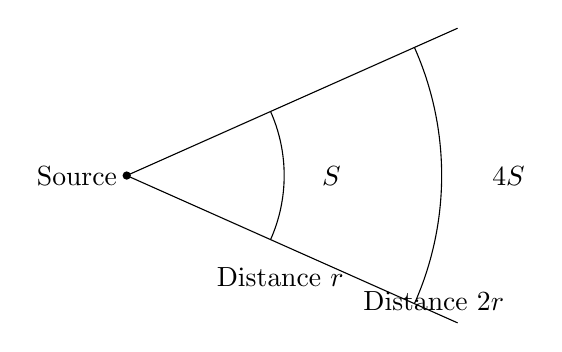
\begin{tikzpicture}[scale=1.0]
  \fill (0,0) circle (1.5pt);
  \node[left] at (0,0) {Source};
  \draw (0,0) -- (24:4.6);
  \draw (0,0) -- (-24:4.6);
  \draw (24:2) arc[start angle=24,end angle=-24,radius=2];
  \draw (24:4) arc[start angle=24,end angle=-24,radius=4];
  \node at (2.6,0) {\(S\)};
  \node at (4.85,0) {\(4S\)};
  \node[below] at (1.95,-1.05) {Distance \(r\)};
  \node[below] at (3.9,-1.35) {Distance \(2r\)};
\end{tikzpicture}
\end{center}

At distance \(r\), the same total falls on receiving area \(S\). Double distance and the rays spread across area \(4S\), doubled in both directions, leaving one-quarter per unit area.

Again state where the analogy works and fails. Gravity resembles spreading light in its geometry of weakening. But photons actually travel, while Newtonian gravity contains no flying gravitational bullets. Instead imagine a notice at every spatial point stating the pull's strength and direction there. This space-filling set of notices is the new concept of a gravitational field. An object feels force not by recognizing another across empty space, but by reading its local notice. Fields may seem unnecessary now, but remember them: in electromagnetism they become an indispensable entity rather than convenient bookkeeping, and later the gravitational field itself will be rewritten.

Mutual attraction and inverse square need a final piece: what does the pull do? Earlier chapters prepared the answer. Force changes momentum and motion state; objects do not need force to maintain motion. Without it, they travel uniformly straight. The question why the Moon does not fall is therefore overturned: it always falls. It would otherwise fly straight away, but gravity pulls it inward a little each instant, bending its track into a closed loop. Circling is not lunar nature but a dynamic balance between gravity and inertia. Similarly, your eraser does not want a circle; the string continually pulls it. Specify this carefully: centripetal force is not a new force alongside gravity and elasticity, but a role. Whichever net force points toward the center and turns the object plays it: gravity for the Moon, string tension for the eraser.

\step{The Model in One Sentence}

\begin{oneline}
Any two masses attract with force proportional to their mass product and inversely proportional to squared distance; celestial bodies continually free-fall while missing the ground, and tides arise from unequal attraction across an object's ends.
\end{oneline}

\step{The Mathematical Translator}

Translate each statement into a calculable expression.

First, mutual inverse-square attraction becomes
\[
F = G\,\frac{m_{1} m_{2}}{r^{2}},
\]
where \(m_{1}\) and \(m_{2}\) are masses, \(r\) is center-to-center distance, and \(G\) is a small measured constant, \(G \approx 6.67\times 10^{-11}\,\mathrm{N\cdot m^{2}/kg^{2}}\). The left asks how hard each object is pulled. Every right-hand term explains what strengthens or weakens the pull: larger masses strengthen it proportionally, greater distance weakens it by inverse square, and \(G\) connects units to nature's actual strength.

Check immediately. Double distance: denominator quadruples, force quarters, matching the flashlight. Infinite separation: force tends to zero, as expected for infinitely distant objects. Zero mass: zero force, no mass to participate. Swap the objects' positions: equal force magnitude and opposite direction, automatically satisfying action and reaction. One check deserves more thought: as \(r\) approaches zero, force diverges. Frightening, but it exposes the hidden point-particle assumption. Real objects have sizes; two basketballs cannot place their centers at zero separation, so the infinity is never encountered. Could a gravitational source truly be compressed very small? Keep that question for the model's limits.

Second, give numbers to the Moon always falling, one of physics' most beautiful cross-checks. At ground level an apple accelerates at \(g \approx 9.8\,\mathrm{m/s^{2}}\). Its distance from Earth's center is approximately Earth's radius, \(R \approx 6.4\times10^{6}\,\mathrm{m}\); the Moon is about \(60 R\) away. If gravity is inverse square, Earth's acceleration at the Moon should be
\[
a_{\text{Moon}} = \frac{g}{60^{2}} = \frac{9.8}{3600} \approx 2.7\times10^{-3}\,\mathrm{m/s^{2}}.
\]
Independently, the Moon's period of about \(27.3\) days and radius \(60R\), inserted into centripetal acceleration \(a = 4\pi^{2}r/T^{2}\), give about \(2.7\times10^{-3}\,\mathrm{m/s^{2}}\) too. Two independent methods, one extrapolating apple fall and one measuring lunar orbit size and rate, give one number. Heaven and Earth were stitched together numerically for the first time. Newton reportedly held this result unpublished for nearly twenty years because he lacked one piece: how could all of large Earth's mass be treated as concentrated at its center?

\begin{mathbridge}
That piece is the shell theorem: a sphere with uniformly spherically symmetric mass distribution attracts every exterior point exactly as though all mass were at its center, while a point inside a spherical shell feels no pull from the shell. Proof integrates attraction from every tiny surface patch. Nearby pieces pull harder but are fewer; distant ones are more numerous but weaker. Integration cancels or combines directional components to produce exact point-mass equivalence. Inverse square is crucial: only it, and its mirror, Hooke's force proportional to distance, allows the miracle. This is why we can confidently use Earth's radius for the Moon calculation and center-to-apple distance for apples.

The same law gives circular orbital speed. A satellite circles Earth at radius \(r\), with gravity providing the inward force:
\[
G\frac{M m}{r^{2}} = m\frac{v^{2}}{r}
\quad\Longrightarrow\quad
v = \sqrt{\frac{GM}{r}}.
\]
The satellite's own \(m\) cancels: at one altitude, a kilogram and a tonne orbit at the same speed. This is the orbital version of all objects falling equally fast. Near Earth, with \(r\) just larger than its radius, substitution gives \(v \approx 7.9\,\mathrm{km/s}\), the first cosmic velocity and the mountaintop cannon's required muzzle speed. Eight kilometers per second is about ten rifle-bullet speeds, explaining why satellites had to wait until the twentieth century.
\end{mathbridge}

The third translation gives Kepler's three laws a home. From data he inferred (1) elliptical planetary orbits with the Sun at one focus; (2) equal areas swept by the planet--Sun line in equal times, hence faster near the Sun and slower far away; and (3) period squared proportional to semimajor axis cubed, \(T^{2} \propto a^{3}\). Newton proved all three follow from inverse-square gravity. Ellipses come from its exact solution; equal areas from an always-central force preserving angular momentum; the third is immediately visible in the circular approximation. Substitute \(v = \sqrt{GM/r}\) into \(T = 2\pi r/v\) and square to get \(T^{2} = 4\pi^{2}r^{3}/(GM)\). Empirical formulas and data patterns became consequences of deeper laws for the first time.

The relation \(T^{2} \propto r^{3}\) has daily engineering uses in communication and navigation satellites. For a satellite to remain above one equatorial point, its period must match Earth's rotation, \(T = 24\) hours. Scale from a low satellite with a roughly ninety-minute period and radius about one Earth radius: \(24\) hours is \(16\) times ninety minutes, so period squared grows \(256\)-fold. Radius cubed must also grow \(256\)-fold, making radius about \(256^{1/3} \approx 6.3\) times as large: roughly 6.3 Earth radii or forty thousand kilometers from the center. Subtract Earth's radius and altitude is around thirty-six thousand kilometers, the actual geostationary altitude that lets satellite dishes point forever one way. Applied to interplanetary travel, these proportions also explain gravitational slingshots: a probe borrows orbital momentum while passing a planet, saving fuel. Voyager was thrown outward through successive encounters this way. Gravitation is an aerospace construction plan here, not an examination exercise.

Fourth, finally, tides. Inverse-square lunar gravity pulls near-side water, Earth's center, and far-side water with three strengths: strongest near, intermediate centrally, weakest far. Relative to Earth's center, near water is pulled extra toward the Moon and bulges that way; far water is pulled less, lags behind the center, and bulges away. Both sides rise. This differential pull across an object is tidal force. It falls off faster than gravity itself: gravity as \(1/r^{2}\), tides as \(1/r^{3}\). That explains why the Moon, with only \(1/27000000\) of the Sun's mass, contributes over twice as much to Earth's tides. It is much closer, and tidal sensitivity to distance has an extra square.

\begin{challenge}
Derive tidal strength with lunar mass \(M\), center-to-center Earth--Moon distance \(d\), and Earth radius \(R\). Lunar acceleration at Earth's center is \(GM/d^{2}\), and at the near point \(GM/(d-R)^{2}\). Expand the latter in \(R\), with \(R \ll d\), retaining first order; the difference is about \(2GMR/d^{3}\). The far point gives equal magnitude in the opposite direction. The factor \(R/d^{3}\) explains proportionality to the stretched object's size and inverse proportionality to distance cubed. This \(1/d^{3}\) dependence matters greatly near extreme celestial objects: closer to the source or larger in size means greater spaghettification risk. It also explains an observation: Earth's tides on the Moon long ago locked lunar rotation to its orbit, keeping the same face toward Earth. This is no coincidence but billions of years of tidal friction.
\end{challenge}

\step{The Model's Limits}

A good model says where it will fail; Newtonian gravity is exemplary.

First, it assumes spherical symmetry or point particles. This works beautifully for planets and moons, but not delicate questions like gravity changing with latitude. Rotation gives Earth an equatorial bulge, and equatorial gravity is weakened both by the slightly greater radius and by rotation's inertial effect, leaving \(g\) about half a percent smaller than at the poles. Newton's law has not failed; the uniform-sphere approximation has reached retirement.

Second, it is inverse-square, instantaneous action at a distance. Newton's formula requires no transmission time: remove the Sun now and Earth immediately flies straight away. Newton found this deeply troubling, writing that unmediated action across empty space was absurd to anyone with a philosophical mind. Yet he chose not to invent hypotheses: let the formula work and leave the mechanism to successors. Einstein repaired this boundary two hundred years later. Gravity propagates at light speed, not instantly, and represents curved spacetime rather than a force. Everyday predictions differ almost imperceptibly, with one famous exception, Mercury. Closest to the Sun and in strongest gravity, its perihelion advances an extra \(43\) arcseconds per century. Newtonian calculations including every planet's pull still miss those \(43\) arcseconds; general relativity supplies them exactly. Newtonian gravity's domain is weak fields and speeds far below light speed. Near black holes or in cosmic large-scale structure, change theories.

Third, common misuses. No gravity in space, hence weightless astronauts: wrong. At a station altitude near four hundred kilometers, gravity is about ninety percent of ground strength. Astronaut and station free-fall together, so neither must support the other. Gravitational acceleration is exactly \(9.8\): only approximately near the surface; altitude, latitude, and underground deposits change it, and geological surveys find minerals through tiny changes. Inverse-square gravity becomes infinite near the source: point-particle approximation fails inside extended objects, and the shell theorem makes gravity weaken linearly with depth inside Earth. Finally, tides merely pull water directly beneath the Moon upward: you now know this confuses average pull with differential pull.

\step{Explaining the Opening Phenomenon}

Return to the sea. Earth and its water form a system pulled by the Moon and Sun. Lunar gravity is strongest near, intermediate at the center, and weakest far away. Fluid seawater responds to the difference, while solid Earth moves approximately under the central pull. In a frame moving with Earth's center, near water gets an extra tug and bulges toward the Moon; far water gets less and lags behind the solid body, bulging away. Two bulges and two low-tide regions remain while Earth rotates underneath daily, taking each coastal place through two high tides. The timetable's twelve hours and twenty-five minutes reflects Earth's rotation plus a small correction for lunar orbital motion.

\begin{center}
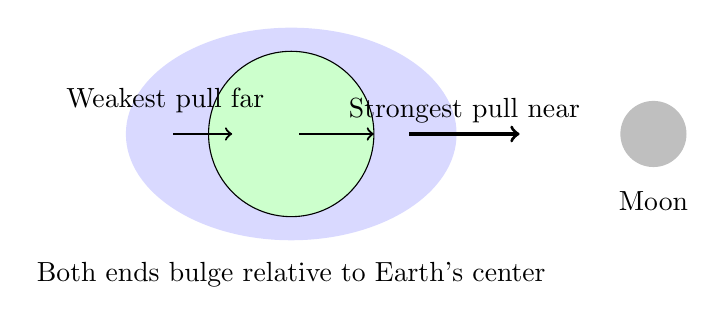
\begin{tikzpicture}[scale=1.0]
  \fill[blue!15] (0,0) ellipse (2.1 and 1.35);
  \fill[green!20] (0,0) circle (1.05);
  \draw (0,0) circle (1.05);
  \fill[gray!50] (4.6,0) circle (0.42);
  \node at (4.6,-0.85) {Moon};
  \draw[->,very thick] (1.5,0) -- (2.9,0);
  \node[above] at (2.2,0.02) {Strongest pull near};
  \draw[->,thick] (0.1,0) -- (1.05,0);
  \draw[->,thick] (-1.5,0) -- (-0.75,0);
  \node[above] at (-1.6,0.15) {Weakest pull far};
  \node[below] at (0,-1.5) {Both ends bulge relative to Earth's center};
\end{tikzpicture}
\end{center}

The three arrows show lunar gravity near, centrally, and far: all toward the Moon, but progressively shorter. Fluid responds to their length differences, not the arrows themselves, so both ends bulge rather than only the near side.

Answer the guesses too. First, (b): gravity does not go around Earth; Earth is pulled harder than the far-side water. Second, revise (a) if you chose it: station gravity is substantial. Weightlessness comes from free fall shared by astronauts, station, water, and pens, all falling with the same acceleration and floating relative to one another. This also explains tens of seconds of weightless training in parabolic aircraft and the rising-stomach feeling on a drop tower. Third: with unlimited strength, the stone circles Earth and returns, ideally perhaps hitting your head if drag is ignored. More likely, sufficient speed sends it away along an open curve forever. Gravity determines that threshold, escape speed, around eleven kilometers per second at the surface. Fourth: one law, the chapter's core.

An everyday echo: why does the Sun contribute to tides? At full and new moons, Sun and Moon nearly align, adding tidal bulges and maximizing range, spring tides. At first and last quarters, their perpendicular bulges partly cancel and minimize range, neap tides. Fishers' lunar-calendar spring tides around the first and fifteenth days come from this. One formula explains apples, Moon, cannonballs, satellites, and fishing conditions: that is the weight of universal.

\step{Thought Experiments and Challenges}

The final idea bridges to the next mountain. Einstein recalled his happiest thought: a person freely falling from a roof feels no weight while falling. Expand this into an experiment:

\begin{thought}[An Elevator with No View Outside]
Imagine a sealed elevator with a scale beneath your feet. At rest on Earth it shows your weight. Cut the cable and both fall freely in Earth's field; the reading becomes zero and you float like a station astronaut. Conversely, place it in gravity-free deep space and propel it upward by rocket at \(9.8\,\mathrm{m/s^{2}}\). The scale again shows your usual weight, and a released apple falls to the floor.

The crucial question: without looking outside, can any physical experiment distinguish free fall in gravity from gravity-free floating, or resting on Earth from rocket acceleration? Newtonian mechanics finds none. Einstein promoted the observation to the equivalence principle: within a sufficiently small region of spacetime, gravity's effects and acceleration's effects are indistinguishable. Follow this road and gravity becomes spacetime geometry rather than force, the story of later chapters. Remember its entrance: all masses fall equally in gravity, and weightlessness means falling with gravity, not its absence.
\end{thought}

This idea works daily in your phone, beyond philosophy. Navigation satellites orbit around twenty thousand kilometers up in weaker gravity, moving near four kilometers per second. Special and general relativity make their atomic clocks gain about thirty-eight microseconds daily against ground clocks. Trivial? Light travels three hundred thousand kilometers per second, so that interval corresponds to over ten kilometers of position error. Without gravitational and relativistic corrections in satellite clock programs, navigation would drift by that amount daily. One satellite links gravity, orbits, atomic clocks, and relativity, previewing why this old friend returns repeatedly later.

\begin{puzzles}
\item Dig a straight tunnel through Earth's center, ignore air resistance and geothermal heat, and jump in from its mouth. Describe the entire motion qualitatively. (Hint: inside Earth at radius \(r\), the shell theorem says only the mass within the sphere of radius \(r\) below you attracts you; outer shells cancel. With approximately uniform density, that mass scales as \(r^{3}\); divide by \(r^{2}\) and force scales as \(r\). You have met a force proportional to displacement and directed toward the center.)

\item Observations show the Moon receding by about \(3.8\) centimeters annually while Earth's spin slows and days lengthen. These are two sides of one process. Use tides to explain what transfers from Earth's rotation to the Moon. (Hint: rotation drags tidal bulges slightly ahead rather than directly toward the Moon. Their pull consequently is not exactly toward Earth's center. What does this tilted force do to the Moon, and its reaction to Earth? Total Earth--Moon angular momentum is conserved.)

\item A geostationary satellite stays fixed relative to the ground about thirty-six thousand kilometers above the equator. Why must it be equatorial, not above Beijing? If Earth's rotation suddenly became twice as slow, how would the synchronous orbit's altitude change? (Hint: gravity alone supplies the required inward pull and always points to Earth's center, so the orbital circle must be centered there. Estimate the change with \(T^{2}\propto r^{3}\), giving direction and approximate factor rather than an exact value.)

\item Tides stretch an astronaut head-to-foot near a black hole, science fiction's spaghettification. Curiously, crossing a supermassive black hole's horizon, like one at a galaxy's center, may feel almost uneventful, while a black hole of a few solar masses tears the astronaut apart before the horizon. Why is the more massive one gentler? (Hint: tides scale as \(M/d^{3}\), horizon radius as \(M\). Express horizon tides in terms of \(M\) and see how they change with increasing \(M\).)
\end{puzzles}
